\documentclass[11pt, a4paper]{article}
\usepackage{graphicx}
\usepackage{wrapfig}
\usepackage{float}
\usepackage{array}
\usepackage{url}
\usepackage{latexsym}
\usepackage{enumitem}
\usepackage{amsmath}
\usepackage{hyperref}
\usepackage{algpseudocode}
\usepackage{listings}
\usepackage{paralist}
\usepackage[utf8]{inputenc}
\usepackage{geometry}
\geometry{a4paper, margin=2cm} 

\setdefaultenum{a)}{i)}{A)}{I)}
\hypersetup{
    colorlinks=true,
    linkcolor=blue,
    citecolor=green,
    filecolor=magenta,
    urlcolor=cyan,
    pdftitle={Subiecte de preadmitere Politehnică - AC-CTI},
    pdfauthor={Numele Autorului},
}
\title{Subiecte de preadmitere Politehnică - secțiunea Informatică}
\author{Cocu Matei-Iulian}
\date{\today}
\begin{document}
\maketitle
\tableofcontents
\newpage


\section{Anul 2025 - Simulare}
\textbf{1.}\newline


\vspace{0.5cm}

\textbf{2.}\newline


\vspace{0.5cm}

\textbf{3.}\newline


\vspace{0.5cm}

\textbf{4.}\newline


\vspace{0.5cm}

\textbf{5.}\newline


\vspace{0.5cm}

\textbf{6.}\newline


\vspace{0.5cm}

\textbf{7.}\newline


\vspace{0.5cm}

\textbf{8.}\newline


\vspace{0.5cm}

\textbf{9.}\newline


\vspace{0.5cm}

\textbf{10.}\newline


\section{Anul 2025}
\textbf{1.}\newline


\vspace{0.5cm}

\textbf{2.}\newline


\vspace{0.5cm}

\textbf{3.}\newline


\vspace{0.5cm}

\textbf{4.}\newline


\vspace{0.5cm}

\textbf{5.}\newline


\vspace{0.5cm}

\textbf{6.}\newline


\vspace{0.5cm}

\textbf{7.}\newline


\vspace{0.5cm}

\textbf{8.}\newline


\vspace{0.5cm}

\textbf{9.}\newline


\vspace{0.5cm}

\textbf{10.}\newline


\section{Anul 2024 - Simulare}
\textbf{1.}\newline
Fie secvența de cod de mai jos. Care dintre instrucțiunile următoare va conduce la o eroare de compilare?
\begin{lstlisting}[language=C++]
struct Produs {
    int pret;
    char cod[10];
} x, y;
int r;
\end{lstlisting}
\begin{lstlisting}
I1) if (x < y) ;
I2) if (x.cod[4] == y.cod[5]) ;
I3) x.cod[1] = y.cod[5];
I4) r=y.pret + x.pret;
I5) x=y;
I6) y.pret++;
\end{lstlisting}
\begin{inparaenum}
    \item I6;
    \item I2 și I3;
    \item I4;
    \item I1 și I6;
    \item I1;
    \item I5;
\end{inparaenum}

\vspace{0.5cm}

\textbf{2.}\newline
În câte moduri se poate colora următorul graf neorientat folosind 4 culori astfel încât 2 noduri adiacente să nu aibă aceeași culoare?
\begin{figure}[h!]
    \centering
    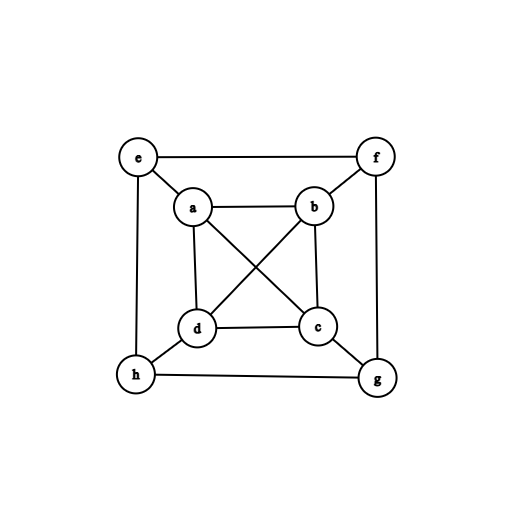
\includegraphics[width=0.6\textwidth]{graph2.png}
\end{figure}
\begin{inparaenum}
    \item 288;
    \item 696;
    \item 625;
    \item 24!;
    \item 120;
    \item 24.
\end{inparaenum}

\vspace{0.5cm}

\textbf{3.}\newline
Se dau $n$ obiecte ($n$ e întreg pozitiv sau $0$) ale căror mase și valori sunt stocate în tablourile unidimensionale de întregi $m$ și, respectiv, $v$ (primul elemente din tablouri se găsește pe poziția $0$). Într-un rucsac se pot transporta obiecte întregi cu masa însumată maxim $C$ (întreg pozitiv sau $0$). Trebuie identificată valoarea maximă ce poate să fie obținută prin adăugarea de obiecte în rucsac, astfel încât masa lor să nu depășească $C$. Procedura descrisă în pseudocod mai jos conține implementarea algoritmului backtracking care returnează soluția. Este considerată dată funcția max care primește 2 parametri întregi și returnează valoarea maximă dintre aceștia. Funcția se apelează cu parametrii: valoarea pentru $C$, tablouri cu valori pentru mase și valori și numărul de obiecte. Completați cu secvența lipsă:
\begin{lstlisting}
int bk(int C, int m[], int v[], int n)
    if(n == 0 || C == 0) return 0;
    if (m[n-1] > C)
        return bk(C, m, v, n-1);
    else
        return _______;
\end{lstlisting}

\begin{inparaenum}
    \item max(v[n-1] + bk(C-m[n-1], m, v, n), bk(C, m, v, n));
    \item max(v[n]+bk(C-m[n], m, v, n-1), bk(C, m, v, n-1));
    \item max(v[n-1]+bk(C-m[n-1], m, v, n-1), bk(C, m, v, n-1));
    \item max(bk(C-m[n-1], m, v, n-1), bk(C, m, v, n-1));
    \item max(v[n]+bk(C-m[n], m, v, n), bk(C, m, v, n));
    \item max(bk(C, m, v, n-1), bk(C, m, v, n-2));
\end{inparaenum}
\vspace{0.5cm}

\textbf{4.}\newline
Numărul de prieteni ai unui număr natural nenul n este egal cu numărul de divizori ai săi. De exemplu, numărul $n=20$ are 6 prieteni, deoarece $20$ are $6$ divizori: ${1,2,4,5,10,20}$. Considerăm un program care citește un șir de k numere naturale de la tastatură și afișează numărul cu cei mai mulți prieteni. Dacă există mai multe numere cu număr maxim de prieteni, se va afișa cel mai mic. Ce va afișa programul considerat dacă se citește la intrare $4 35 8 10 4$?
\begin{inparaenum}
    \item 35;
    \item 10;
    \item 1;
    \item 0;
    \item 8;
    \item 4.
\end{inparaenum}

\vspace{0.5cm}

\textbf{5.}\newline
Specificați ce afișează următoarea secvență de cod:
\begin{lstlisting}
char c[12]="Politehnica";
int i, j;
for(i=0; i<strlen(c); i++)
{
    if (i == 3)
        c[i] = 'n';
    for(j=0; j<strlen(c); j++)
        if(c[j]=='n') break;
    printf("%d", j);
    /* cout<<j; // versiunea C++ */
}
\end{lstlisting}
\begin{inparaenum}
    \item 3333333777;
    \item 7333333333;
    \item 77733333333;
    \item 99933333333;
    \item 33333333333;
    \item 99999999999.
\end{inparaenum}

\vspace{0.5cm}

\textbf{6.}\newline
Care este rezultatul întreg întors de funcția scrisă mai jos în pseudocod, dacă este apelată cu valoarea $3$ pentru parametrul $a$ întreg și $10$ pentru parametrul $n$ întreg? S-a notat cu $a\%b$ restul împărțirii numărului natural $a$ la numărul natural nenul $b$ și cu $[a]$ partea întreagă a numărului real $a$.
\begin{lstlisting}[language=C++]
int f(int a, int n) {
    if (n == 0) return 1;
    else if (n % 2 == 0) return f(a, n/2) * f(a, n/2);
    else return a * f(a, n/2) * f(a, n/2);
}
\end{lstlisting}
\begin{inparaenum}
    \item 39366;
    \item 243;
    \item 486;
    \item 177147;
    \item 59049;
    \item 19683.
\end{inparaenum}

\vspace{0.5cm}

\textbf{7.}\newline
Un arbore cu 11 noduri, numerotate de la 1 la 11, este memorat cu ajutorul vectorului  de "tați" $t={2,5,5,3,0,6,2,4,6,6,2,3}$. Mulțimea tuturor ascendenților nodului 8 este:
\begin{inparaenum}
    \item \{ 1,2,5,6 \};
    \item \{ 1,2,5,6,10 \};
    \item \{ 2,3,6 \};
    \item \{ 6 \};
    \item \{ 2,5,6 \};
    \item \{ 2,5 \}.
\end{inparaenum} 

\vspace{0.5cm}

\textbf{8.}\newline
Se consideră o hartă sub forma unei matrice $4\times4$. Dacă cineva pleacă de pe poziția $(1,1)$ și vrea să ajungă în celula $(4,4)$, se poate muta doar pe linii sau coloane cu numere mai mari și poate sări oricât de multe în ambele direcții. deci poate ajunge inclusiv direct din $(1,1)$ în $(4,4)$, în câte moduri distincte poate face acest lucru?
\begin{inparaenum}
    \item 76;
    \item 128;
    \item 256;
    \item 63;
    \item 252;
    \item 64.
\end{inparaenum}
\vspace{0.5cm}

\textbf{9.}\newline
Fie vectorul $V={a,a,a,b,b,c,d,d,d,d}$, cu $a, b, c$ și $d$ numere naturale diferite. Câte permutări distincte ale lui $V$ sunt posibile?
\begin{inparaenum}
    \item 75600;
    \item 3628800;
    \item 12600;
    \item 5040;
    \item 7560;
    \item 138600.
\end{inparaenum}

\vspace{0.5cm}

\textbf{10.}\newline
Se definește o secvență de numere folosind recurența: $D_0=a, D_1=b, D_n=suma_cifre(D_{n-1}+D_{n-2})$, pentru $n>=2$, unde $suma\_cifre$ este o funcție care calculează suma cifrelor unui număr natural. Un program primește ca date de intrare $a, b$ și $n$ și afișează termenul $D_n$. Pentru două execuții consecutive ale programului considerat se dau ca date de intrare, $1 1 11$, respectiv $5 2024 8$. Care sunt rezultatele afișate?
\begin{inparaenum}
    \item 2 și 4;
    \item 1 și 2024;
    \item 9 și 8;
    \item 1 și 5;
    \item 8 și 7;
    \item 7 și 7.
\end{inparaenum}


\section{Anul 2024}
\textbf{1.}\newline
Fie vectorul $v={4,7,1,5,8,9,4,2,1,1}$. Primul element este pe poziția 0. Care este valoarea expresiei $v[v[v[0]]] + v[v[0]] + v[0]$?
\begin{inparaenum}
    \item 20;
    \item 13;
    \item 14;
    \item 6;
    \item 11;
    \item 17.
\end{inparaenum}

\vspace{0.5cm}

\textbf{2.}\newline
Se dă o matrice cu 3 linii și 3 coloane. Pornim din celula de start $(1,1)$ și vrem să ajungem în celula destinație $(3,3)$
\begin{inparaenum}
    \item ;
    \item ;
    \item ;
    \item ;
    \item ;
    \item .
\end{inparaenum}

\vspace{0.5cm}

\textbf{3.}\newline

\begin{inparaenum}
    \item ;
    \item ;
    \item ;
    \item ;
    \item ;
    \item .
\end{inparaenum}


\vspace{0.5cm}

\textbf{4.}\newline

\begin{inparaenum}
    \item ;
    \item ;
    \item ;
    \item ;
    \item ;
    \item .
\end{inparaenum}

\vspace{0.5cm}

\textbf{5.}\newline

\begin{inparaenum}
    \item ;
    \item ;
    \item ;
    \item ;
    \item ;
    \item .
\end{inparaenum}

\vspace{0.5cm}

\textbf{6.}\newline

\begin{inparaenum}
    \item ;
    \item ;
    \item ;
    \item ;
    \item ;
    \item .
\end{inparaenum}

\vspace{0.5cm}

\textbf{7.}\newline

\begin{inparaenum}
    \item ;
    \item ;
    \item ;
    \item ;
    \item ;
    \item .
\end{inparaenum}

\vspace{0.5cm}

\textbf{8.}\newline

\begin{inparaenum}
    \item ;
    \item ;
    \item ;
    \item ;
    \item ;
    \item .
\end{inparaenum}

\vspace{0.5cm}

\textbf{9.}\newline

\begin{inparaenum}
    \item ;
    \item ;
    \item ;
    \item ;
    \item ;
    \item .
\end{inparaenum}

\vspace{0.5cm}

\textbf{10.}\newline

\begin{inparaenum}
    \item ;
    \item ;
    \item ;
    \item ;
    \item ;
    \item .
\end{inparaenum}



\section{Anul 2023}
\textbf{1.}\newline

\begin{inparaenum}
    \item ;
    \item ;
    \item ;
    \item ;
    \item ;
    \item .
\end{inparaenum}

\vspace{0.5cm}

\textbf{2.}\newline

\begin{inparaenum}
    \item ;
    \item ;
    \item ;
    \item ;
    \item ;
    \item .
\end{inparaenum}

\vspace{0.5cm}

\textbf{3.}\newline

\begin{inparaenum}
    \item ;
    \item ;
    \item ;
    \item ;
    \item ;
    \item .
\end{inparaenum}

\vspace{0.5cm}

\textbf{4.}\newline

\begin{inparaenum}
    \item ;
    \item ;
    \item ;
    \item ;
    \item ;
    \item .
\end{inparaenum}

\vspace{0.5cm}

\textbf{5.}\newline

\begin{inparaenum}
    \item ;
    \item ;
    \item ;
    \item ;
    \item ;
    \item .
\end{inparaenum}

\vspace{0.5cm}

\textbf{6.}\newline

\begin{inparaenum}
    \item ;
    \item ;
    \item ;
    \item ;
    \item ;
    \item .
\end{inparaenum}

\vspace{0.5cm}

\textbf{7.}\newline

\begin{inparaenum}
    \item ;
    \item ;
    \item ;
    \item ;
    \item ;
    \item .
\end{inparaenum}

\vspace{0.5cm}

\textbf{8.}\newline

\begin{inparaenum}
    \item ;
    \item ;
    \item ;
    \item ;
    \item ;
    \item .
\end{inparaenum}

\vspace{0.5cm}

\textbf{9.}\newline

\begin{inparaenum}
    \item ;
    \item ;
    \item ;
    \item ;
    \item ;
    \item .
\end{inparaenum}

\vspace{0.5cm}

\textbf{10.}\newline

\begin{inparaenum}
    \item ;
    \item ;
    \item ;
    \item ;
    \item ;
    \item .
\end{inparaenum}


\section{Anul 2022}
\textbf{1.}\newline

\begin{inparaenum}
    \item ;
    \item ;
    \item ;
    \item ;
    \item ;
    \item .
\end{inparaenum}

\vspace{0.5cm}

\textbf{2.}\newline

\begin{inparaenum}
    \item ;
    \item ;
    \item ;
    \item ;
    \item ;
    \item .
\end{inparaenum}

\vspace{0.5cm}

\textbf{3.}\newline

\begin{inparaenum}
    \item ;
    \item ;
    \item ;
    \item ;
    \item ;
    \item .
\end{inparaenum}

\vspace{0.5cm}

\textbf{4.}\newline

\begin{inparaenum}
    \item ;
    \item ;
    \item ;
    \item ;
    \item ;
    \item .
\end{inparaenum}

\vspace{0.5cm}

\textbf{5.}\newline

\begin{inparaenum}
    \item ;
    \item ;
    \item ;
    \item ;
    \item ;
    \item .
\end{inparaenum}

\vspace{0.5cm}

\textbf{6.}\newline

\begin{inparaenum}
    \item ;
    \item ;
    \item ;
    \item ;
    \item ;
    \item .
\end{inparaenum}

\vspace{0.5cm}

\textbf{7.}\newline

\begin{inparaenum}
    \item ;
    \item ;
    \item ;
    \item ;
    \item ;
    \item .
\end{inparaenum}

\vspace{0.5cm}

\textbf{8.}\newline

\begin{inparaenum}
    \item ;
    \item ;
    \item ;
    \item ;
    \item ;
    \item .
\end{inparaenum}

\vspace{0.5cm}

\textbf{9.}\newline

\begin{inparaenum}
    \item ;
    \item ;
    \item ;
    \item ;
    \item ;
    \item .
\end{inparaenum}

\vspace{0.5cm}

\textbf{10.}\newline

\begin{inparaenum}
    \item ;
    \item ;
    \item ;
    \item ;
    \item ;
    \item .
\end{inparaenum}


\section{Anul 2021}

% \begin{figure}[h!]
%     \centering
%     \includegraphics[width=0.6\textwidth]{placeholder.png}
% \end{figure}

\end{document}